% \documentclass{article}

% \documentclass{book}

\documentclass{report}

\usepackage{start/init}

\begin{document} % Bắt đầu

%%%%%%%%%%%%%%%%%%%%%%%%%%%%%%%%%%
 

% \begin{titlepage}

    \begin{tikzpicture}[remember picture, overlay]\draw [line width = 3pt]($ (current page.north west) + (3.0cm, - 2.5cm)$)rectangle($ (current page.south east) + (- 2.5cm, 2.5cm)$);\draw [line width = 0.5pt]($ (current page.north west) + (3.1cm, - 2.6cm)$)rectangle($ (current page.south east) + (- 2.6cm, 2.6cm)$);\end{tikzpicture}
    
    \begin{center}
    
    \vspace{- 0.4cm}
    
    \textbf{ĐẠI HỌC BÁCH KHOA HÀ NỘI} \\
    
    \textbf{VIỆN TOÁN ỨNG DỤNG VÀ TIN HỌC} \\
    
    \textbf{******}
    
    \vspace{0.8cm}
    
    \begin{figure}[H]
    
    \centering
    
    
\includegraphics[scale = .5]{pictures/hust/main.png}
    
    \end{figure}
    
    \vspace{0.7cm}
    
    \textbf{\fontsize{16pt}{30pt}\selectfont {BÁO CÁO ĐỒ ÁN II}} \\
    
    \textbf{\fontsize{10pt}{24pt}\selectfont {CHUYÊN NGÀNH: TOÁN TIN}}
    
    \vspace{1cm}
    
    \textbf{\fontsize{16pt}{30pt}\selectfont {ĐỀ TÀI:}} \\
    
    % \textbf{\fontsize{19pt}{24pt}\selectfont {Xây dựng kiến trúc vi dịch vụ cho \\ bài toán hóa đơn điện tử}} \\
    
    \textbf{\fontsize{20pt}{24pt}\selectfont {Sử dụng thiết kế hướng miền \\ xây dựng kiến trúc vi dịch vụ cho \\ bài toán hóa đơn điện tử}} \\
    
    \end{center}
    
    \vspace{0.7cm}
    
    \hspace{2.6cm}\begin{minipage}{0.8\textwidth}
    
    \textbf{\fontsize{10pt}{24pt}\selectfont {Giảng viên hướng dẫn: TS. Vũ Thành Nam}}
    
    \end{minipage}
    
    \vspace{0.7cm}
    
    \hspace{3cm}\begin{minipage}{0.7\textwidth}
    
    \begin{tabular}{l l l}
    
    \textbf{\fontsize{10pt}{24pt}\selectfont {Sinh viên thực hiện}} & \textbf{\fontsize{10pt}{24pt}\selectfont {Vũ Văn Nghĩa}} \\
    
    \textbf{\fontsize{10pt}{24pt}\selectfont {Mã số sinh viên}} & \textbf{\fontsize{10pt}{24pt}\selectfont {20206205}} \\
    
    \textbf{\fontsize{10pt}{24pt}\selectfont {Lớp}} & \textbf{\fontsize{10pt}{24pt}\selectfont {Toán Tin 02 - K65}} \\
    
    \end{tabular}
    
    \end{minipage}
    
    \vspace{0.5cm}
    
    \begin{center}
    
    \textbf{Hà Nội, \the\month~/~\the\year}
    
    \end{center}
    
    \end{titlepage}
    
     

% % Trang trắng không có nội dung và không có số trang

\pagestyle{empty}

\thispagestyle{empty}

\mbox{} % Một hộp rỗng để trang không bị trắng toàn bộ

\newpage



% \newpage

\begin{center}

{\bfseries NHẬN XÉT CỦA GIẢNG VIÊN HƯỚNG DẪN}

\end{center}

\begin{enumerate}

\item Mục đích và nội dung của đồ án:

\vspace{20ex} % Thêm khoảng cách dọc

\item 	Kết quả đạt được:

\vspace{20ex} % Thêm khoảng cách dọc

\item 	Ý thức làm việc của sinh viên:

\vspace{20ex} % Thêm khoảng cách dọc

\end{enumerate}

\hspace{0.4\textwidth}\begin{minipage}{0.5\textwidth}

\noindent\begin{center}

\textit{Hà Nội, \today} \\

\textbf{Giảng viên hướng dẫn} \\

\textit{(Ký và ghi rõ họ tên)}

\vspace{2cm}

\textbf{TS. Vũ Thành Nam}

\end{center}

\end{minipage}

\pagestyle{empty}

\newpage



% 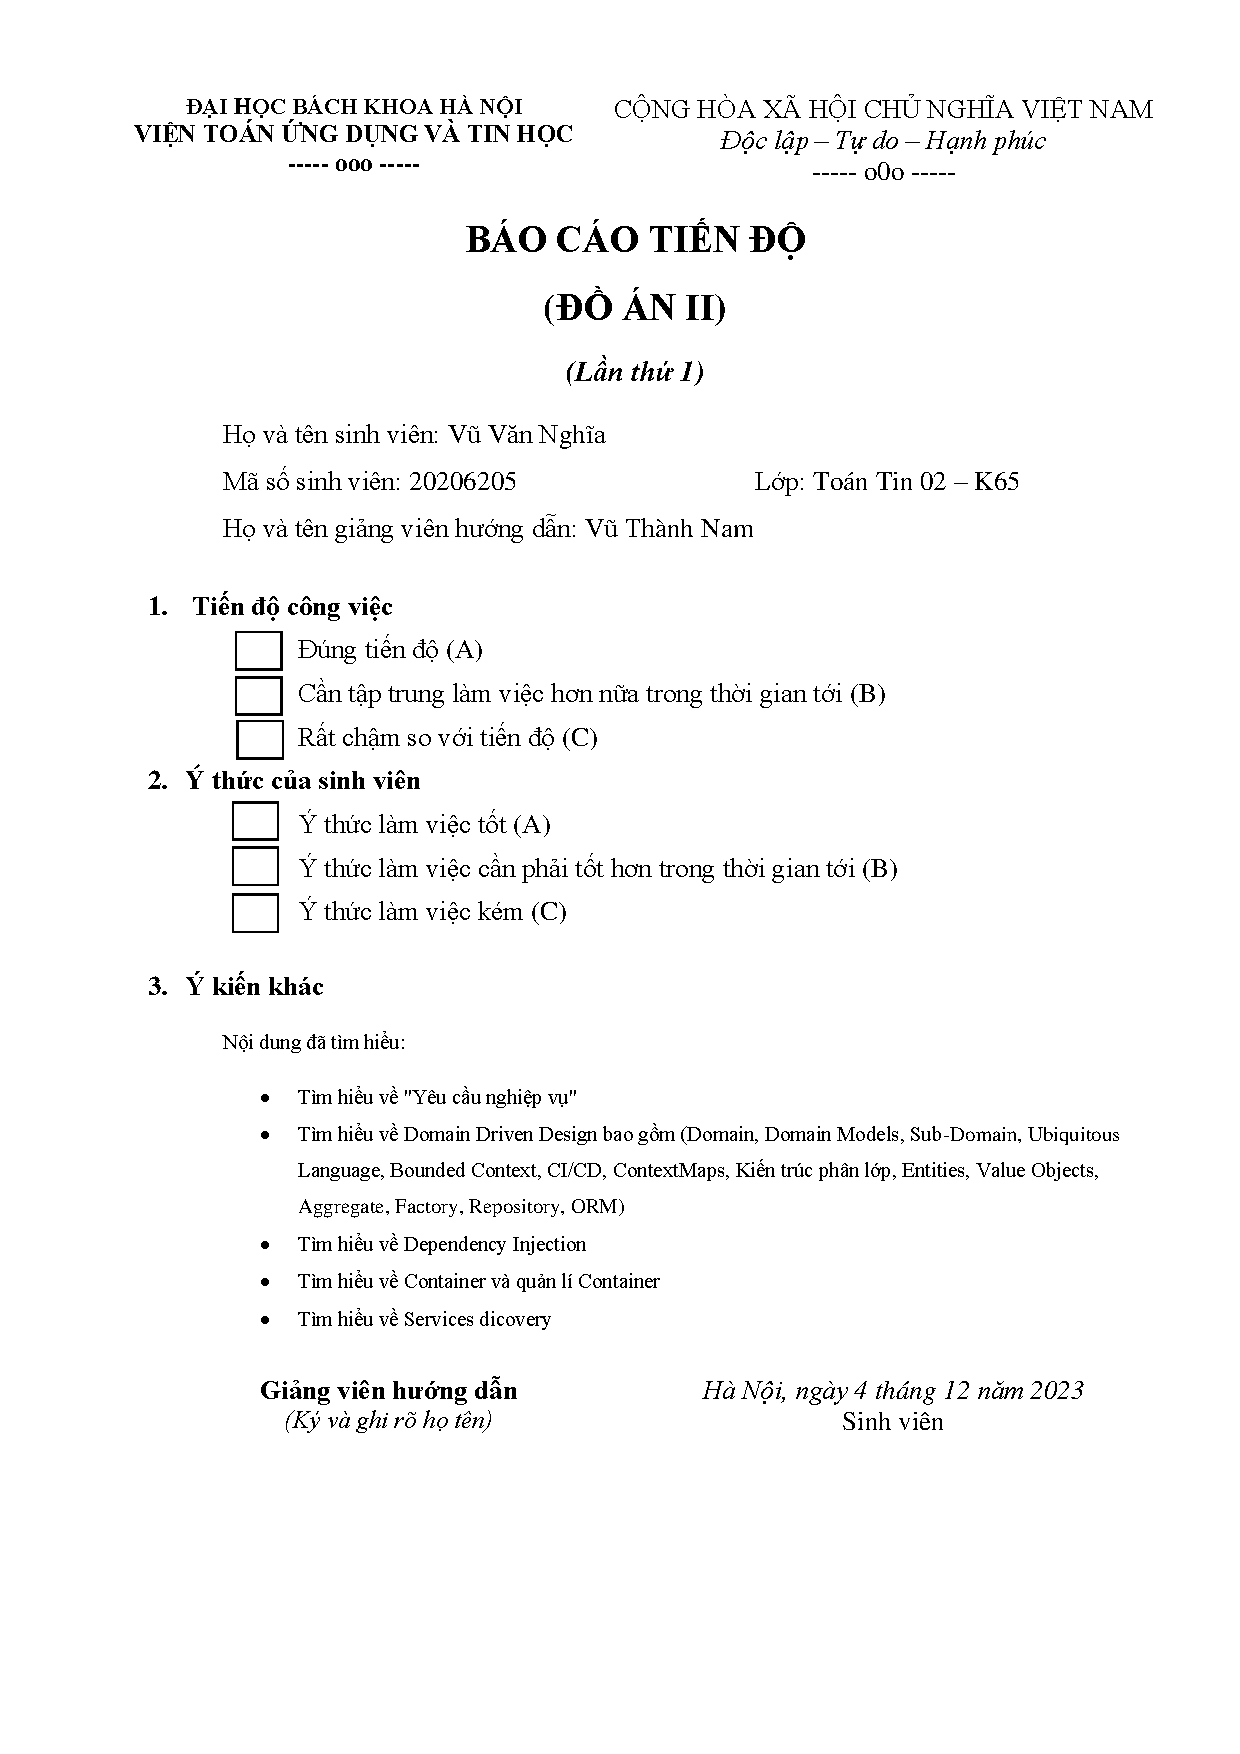
\includepdf[pages = -]{contents/bao_cao_tien_do_1.pdf}

% 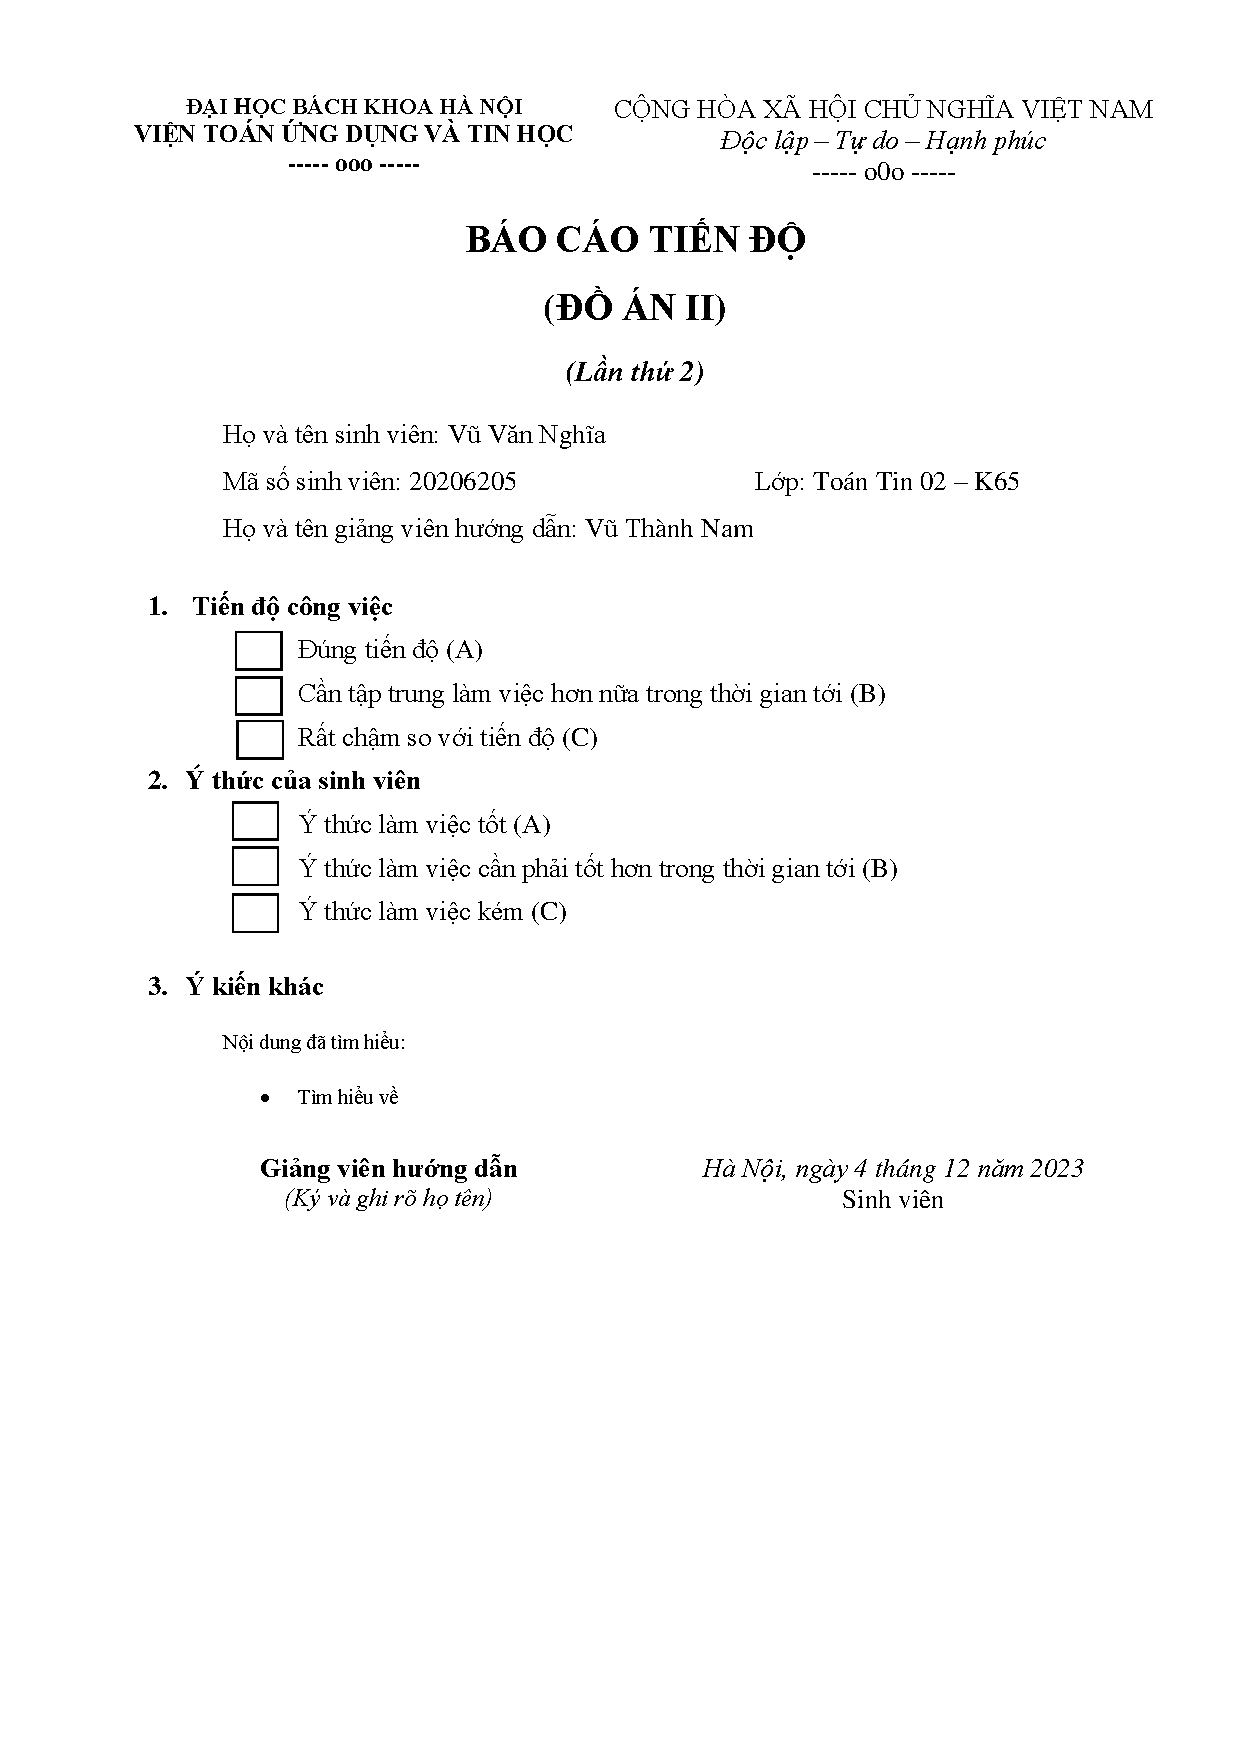
\includepdf[pages = -]{contents/bao_cao_tien_do_2.pdf}

% \newpage

\renewcommand*\contentsname{\centering MỤC LỤC}

\tableofcontents
\setcounter{page}{0}  
\newpage

 







% \newpage

\section*{\centering LỜI CẢM ƠN}

\addcontentsline{toc}{section}{LỜI CẢM ƠN}

\blindtext % Tạo  văn bản ngẫu nhiên

\newpage



% \newpage

\section*{\centering LỜI MỞ ĐẦU}

\addcontentsline{toc}{section}{LỜI MỞ ĐẦU}

\blindtext % Tạo  văn bản ngẫu nhiên

\newpage

% \newpage

\section*{\centering TÓM TẮT NỘI DUNG ĐỒ ÁN}

\addcontentsline{toc}{section}{TÓM TẮT NỘI DUNG ĐỒ ÁN}

\blindtext % Tạo  văn bản ngẫu nhiên

\newpage

% \newpage

\section*{\centering ĐÁNH GIÁ VÀ THẢO LUẬN}

\addcontentsline{toc}{section}{ĐÁNH GIÁ VÀ THẢO LUẬN}

\blindtext % Tạo  văn bản ngẫu nhiên

\newpage

% \newpage

\section*{\centering DANH SÁCH BẢNG}

\addcontentsline{toc}{section}{DANH SÁCH BẢNG}

\makeatletter

\renewcommand\listoftables{

\@starttoc{lot}

}

\makeatother

\listoftables

\newpage

% \newpage

\section*{\centering DANH SÁCH HÌNH ẢNH}

\addcontentsline{toc}{section}{DANH SÁCH HÌNH ẢNH}

\makeatletter

\renewcommand\listoffigures{

\@starttoc{lof}

}

\makeatother

\listoffigures

\newpage



% \newpage

\section*{\centering DANH SÁCH CÁC CỤM TỪ VIẾT TẮT}

\addcontentsline{toc}{section}{DANH SÁCH CÁC CỤM TỪ VIẾT TẮT}

% @sau

\begin{table}[h]

\centering

\begin{tabular}{|c|c|c|c|}

\hline

STT & Từ viết tắt & Từ viết đầy đủ & Mô tả \\

\hline

Dong1 & Dong1 & Cot1 & Cot2 \\

\hline

Dong2 & Dong2 & Cot1 & Cot2 \\

\hline

\end{tabular}

\end{table}

\newpage

% API; Application Programming Interface; Giao diện lập trình ứng dụng

% CI/CD; Continuous Integration (CI) and Continuous Delivery (CD) ; Quá trình tích hợp và chuyển giao liên tục

% thiết kế hướng miền ; thiết kế hướng miền; Kỹ thuật thiết kế theo hướng miền

% DI; Dependency Injection; Cơ chế tiêm sự phụ thuộc giữa các đối tượng

% HTTP; Hypertext Transfer Protocol; Giao thức truyền tải siêu văn bản

% JSON; JavaScript Object Notation; Một kiểu dữ liệu mở rộng của JavaScript

% ORM; Object Relational Mapping; Một kỹ thuật ánh xạ các đối tượng lập trình với từng bảng trong CSDL quan hệ

% Cơ sở dữ liệu ; CSDL ;

% Tạo (Create), Đọc (Read), Sửa (Update), Xóa (Delete) ; CRUD ;

% Kubernetes ; K8s ; kubernetes

% Số điện thoại ; SĐT ;

% UML

% MVC; Model View Controller; Một mẫu thiết kế ứng dụng

% SQL

SOA; Service Oriented Architecture; Kiến trúc hướng dịch vụ

SOAP; Simple Object Access Protocol; Một giao thức để truy cập dịch vụ web

SPA; Single Page Application; Kiểu ứng dụng một trang

REST; Representational State Transfer; Một tiêu chuẩn thiết kế các API sử dụng cho các dịch vụ web

URL; Uniform Resource Locator ; Địa chỉ định vị tài nguyên trên Internet

XML; Extensible Markup Language; Ngôn ngữ đánh dấu mở rộng

% TCT ; TCT ;

Người nộp thuế ; NNT ;

Mã số thuế ; MST ;

Hóa đơn điện tử ; HĐĐT ;

Cơ quan thuế ; CQT ;

Công nghệ thông tin ; CNTT ;



% \newpage

\section*{\centering DANH SÁCH CÁC THUẬT NGỮ}

\addcontentsline{toc}{section}{DANH SÁCH CÁC THUẬT NGỮ}

% @sau

% @sau

\begin{table}[h]

\centering

\begin{tabular}{|c|c|c|}

\hline

STT & Tiếng Anh & Tiếng Việt \\

\hline

Dong1 & Dong1 & Cot2 \\

\hline

Dong2 & Dong2 & Cot2 \\

\hline

\end{tabular}

\end{table}

\newpage

% kiến trúc nguyên khối, kiến trúc nguyên khối

% kiến trúc nguyên khối, kiến trúc nguyên khối

% kiến trúc vi dịch, kiến trúc vi dịch

% kiến trúc vi dịch, kiến trúc vi dịch

% kiến trúc vi dịch, kiến trúc vi dịch

% kiến trúc vi dịch, kiến trúc vi dịch

% thiết kế hướng miền, thiết kế hướng miền

% thiết kế hướng miền, thiết kế hướng miền

1 thiết kế hướng miền

Thiết kế hướng lĩnh vực

2 Domain (không dịch)

3 Abstraction Trừu tượng

4 chuyên gia ngành

%%%%%%%%%%%%%%%%%%%%%%%%%%%%%%%%%%


% \chapter{Giới thiệu}

% Trong thời đại ngày nay, nhu cầu phát triển ứng dụng và hệ thống ngày càng tăng, đặt ra thách thức đối với kiến trúc phần mềm. Kiến trúc nguyên khối đã phục vụ hiệu quả trong quá khứ, nhưng kiến trúc này bắt đầu gặp khó khăn khi đối mặt với sự phức tạp, khả năng mở rộng và khả năng đáp ứng linh hoạt với sự thay đổi nhanh chóng trong yêu cầu kinh doanh.

Kiến trúc vi dịch vụ là giải pháp cho những thách thức trên. Kiến trúc vi dịch vụ chia dự án thành những dịch vụ nhỏ độc lập, mỗi dịch vụ chịu trách nhiệm về một chức năng cụ thể. Từ đó, dự án giảm sự phức tạp, tăng tính linh hoạt và dễ dàng quản lý.

Việc vận dụng kết hợp giữa kiến trúc vi dịch vụ và thiết kế hướng miền là một cách tiếp cận toàn diện, giúp xác định và tổ chức các dịch vụ dựa trên việc hiểu rõ về lĩnh vực kinh doanh. Thiết kế hướng miền xây dựng mô hình dựa trên yêu cầu nghiệp vụ thực tế, từ đó dự án phản ánh đúng các quy trình kinh doanh.




% \section{Giới thiệu về bài toán hóa đơn điện tử}

% Bài toán hóa đơn điện tử là một phần quan trọng của quá trình chuyển đổi số. Trong quá khứ, mọi người thường sử dụng hóa đơn giấy truyền thống. Ngày nay, khi có quy định kế toán và quản lý tài chính, hóa đơn điện tử đã trở nên phổ biến giúp giảm bớt sự phụ thuộc vào giấy tờ. Cùng với sự phát triển của khoa học công nghệ đã giúp quản lý hiệu quả công việc và tối ưu hóa quy trình kế toán và tài chính.




% \emph{Theo em tìm hiểu có các khái niệm và căn cứ pháp lý liên quan sau đây:}

% \subsection{Hóa đơn}

% \emph{Theo quy định tại khoản 1 Điều 3 Nghị định 123/2020/NĐ - CP:}

% %%%%%%%%%%%%%%%%%%%%%%%%%%%%%%%%%%%%%!

Hóa đơn là chứng từ kế toán do tổ chức, cá nhân bán hàng hóa, cung cấp dịch vụ lập, ghi nhận thông tin bán hàng hóa, cung cấp dịch vụ. Hóa đơn được thể hiện theo hình thức hóa đơn điện tử hoặc hóa đơn do cơ quan thuế đặt in.

%%%%%%%%%%%%%%%%%%%%%%%%%%%%%%%%%%%%%!



% \subsection{Hóa đơn điện tử}

% \emph{Theo quy định tại khoản 2 Điều 3 Nghị định 123/2020/NĐ - CP:}

% %%%%%%%%%%%%%%%%%%%%%%%%%%%%%%%%%%%%%!

Hóa đơn điện tử là hóa đơn có mã hoặc không có mã của cơ quan thuế được thể hiện ở dạng dữ liệu điện tử do tổ chức, cá nhân bán hàng hóa, cung cấp dịch vụ lập bằng phương tiện điện tử để ghi nhận thông tin bán hàng hóa, cung cấp dịch vụ theo quy định của pháp luật về kế toán, pháp luật về thuế, bao gồm cả trường hợp hóa đơn được khởi tạo từ máy tính tiền có kết nối chuyển dữ liệu điện tử với cơ quan thuế, trong đó:

a. Hóa đơn điện tử có mã của cơ quan thuế là hóa đơn điện tử được cơ quan thuế cấp mã trước khi tổ chức, cá nhân bán hàng hóa, cung cấp dịch vụ gửi cho người mua. Mã của cơ quan thuế trên hóa đơn điện tử bao gồm số giao dịch là một dãy số duy nhất do hệ thống của cơ quan thuế tạo ra và một chuỗi ký tự được cơ quan thuế mã hóa dựa trên thông tin của người bán lập trên hóa đơn.

b. Hóa đơn điện tử không có mã của cơ quan thuế là hóa đơn điện tử do tổ chức bán hàng hóa, cung cấp dịch vụ gửi cho người mua không có mã của cơ quan thuế.

%%%%%%%%%%%%%%%%%%%%%%%%%%%%%%%%%%%%%!



% \subsection{Bắt buộc sử dụng hóa đơn điện tử từ 01/07/2022}

% \emph{Theo quy định tại khoản 1 Điều 59 Nghị định 123/2020/NĐ - CP:}

% %%%%%%%%%%%%%%%%%%%%%%%%%%%%%%%%%%%%%!

Nghị định này có hiệu lực thi hành kể từ ngày 01 tháng 7 năm 2022, khuyến khích cơ quan, tổ chức, cá nhân đáp ứng điều kiện về hạ tầng công nghệ thông tin áp dụng quy định về hóa đơn, chứng từ điện tử của Nghị định này trước ngày 01 tháng 7 năm 2022.

%%%%%%%%%%%%%%%%%%%%%%%%%%%%%%%%%%%%%!

% Chủ đề đồ án

Theo quy định, tất cả các doanh nghiệp, tổ chức và hộ kinh doanh đều bắt buộc phải chuyển từ sử dụng hóa đơn giấy sang hóa đơn điện tử bắt đầu từ tháng 07/2022. Vì vậy, nhu cầu sử dụng và xử lý hóa đơn điện tử trở nên rất lớn. Do đó ở đồ án này, em chọn chủ đề về quản lý hóa đơn điện tử.

% \subsection{Lưu trữ hóa đơn điện tử}

% \emph{Theo quy định tại khoản 1 Điều 11 Thông tư 32/2011/TT - BTC:}

%%%%%%%%%%%%%%%%%%%%%%%%%%%%%%%%%%%%%!

Người bán, người mua hàng hoá, dịch vụ sử dụng hóa đơn điện tử để ghi sổ kế toán, lập báo cáo tài chính phải lưu trữ hóa đơn điện tử theo thời hạn quy định của Luật Kế toán. Trường hợp hóa đơn điện tử được khởi tạo từ hệ thống của tổ chức trung gian cung cấp giải pháp hóa đơn điện tử thì tổ chức trung gian này cũng phải thực hiện lưu trữ hóa đơn điện tử theo thời hạn nêu trên.

%%%%%%%%%%%%%%%%%%%%%%%%%%%%%%%%%%%%%!

\emph{Theo quy định tại khoản 5 Điều 41 Luật số 88/2015/QH13:}

%%%%%%%%%%%%%%%%%%%%%%%%%%%%%%%%%%%%%!

1. Tài liệu kế toán phải được lưu trữ theo thời hạn sau đây:

a. Ít nhất là 05 năm đối với tài liệu kế toán dùng cho quản lý, điều hành của đơn vị kế toán, gồm cả chứng từ kế toán không sử dụng trực tiếp để ghi sổ kế toán và lập báo cáo tài chính.

b. Ít nhất là 10 năm đối với chứng từ kế toán sử dụng trực tiếp để ghi sổ kế toán và lập báo cáo tài chính, sổ kế toán và báo cáo tài chính năm, trừ trường hợp pháp luật có quy định khác.

c. Lưu trữ vĩnh viễn đối với tài liệu kế toán có tính sử liệu, có ý nghĩa quan trọng về kinh tế, an ninh, quốc phòng.

%%%%%%%%%%%%%%%%%%%%%%%%%%%%%%%%%%%%%!

% Thời gian lưu trữ

Như vậy, hóa đơn điện tử sẽ được lưu trữ trên hệ thống hóa đơn điện tử của nhà cung cấp hoặc doanh nghiệp với thời gian lưu trữ ít nhất là 10 năm theo quy định của pháp luật.



% \subsection{Một số lợi ích của hóa đơn điện tử}

% \emph{Một số lợi ích của hóa đơn điện tử:}

\begin{itemize}

\item Tuân thủ các quy định về thuế và pháp luật.

\item Thể hiện tính minh bạch: bảo vệ quyền lợi của người mua và người bán.

\item Giúp tiết kiệm chi phí in ấn, lưu trữ và bảo quản.

\item Loại bỏ rủi ro cháy, hỏng hoặc mất và dễ dàng sao lưu.

\item Dễ dàng tra cứu, phát hành, quản lý, tạo báo cáo và giảm thủ tục giấy tờ.

\item Giúp theo dõi tình hình tài chính của công ty (doanh thu, chi phí, lợi nhuận).

\end{itemize}



%%%%%%%%%%%%%%%%%%%%%%%%%%%%%%%%%%
% \section{Giới thiệu về kiến trúc vi dịch vụ}


% \subsection{Kiến trúc nguyên khối}

% Trước khi kiến trúc vi dịch vụ trở nên phổ biến, kiến trúc nguyên khối đã được áp dụng rộng rãi trong kiến trúc phần mềm truyền thống. Kiến trúc nguyên khối là kiến trúc phần mềm trong đó tất cả các thành phần của dự án được xây dựng thành một đơn vị triển khai duy nhất.

Trong kiến trúc nguyên khối, bất kỳ thay đổi nào đối với một thành phần đều yêu cầu toàn bộ dự án phải được kiểm thử và triển khai lại. Dẫn đến tốc độ phát triển chậm và thiếu khả năng mở rộng.

Ví dụ: Mô hình MVC (Model - View - Controller) là một trong những dạng của kiến trúc nguyên khối. Trong mô hình này, ứng dụng được chia thành ba thành phần chính:

\begin{itemize}

\item Mô hình (Model): Đại diện cho dữ liệu và logic xử lý dữ liệu.

\item Giao diện (View): Đại diện cho giao diện người dùng.

\item Bộ điều khiển (Controller): Nhận yêu cầu người dùng thông qua View, sau đó tương tác với Model để làm việc với dữ liệu.

\end{itemize}



% \subsection{Kiến trúc vi dịch vụ}

% Kiến trúc vi dịch vụ chia dự án thành các thành phần nhỏ hơn được gọi là các dịch vụ.

Mỗi dịch vụ tập trung vào một khả năng kinh doanh cụ thể.

Các dịch vụ độc lập và giao tiếp với nhau thông qua hạ tầng mạng.

Trong thực tế, nhiều dự án thường chuyển đổi một cách dần dần từ kiến trúc nguyên khối sang kiến trúc vi dịch vụ.

\begin{figure}[H]

% Khi nào Vẽ lại chất lượng cao hơn

\centering

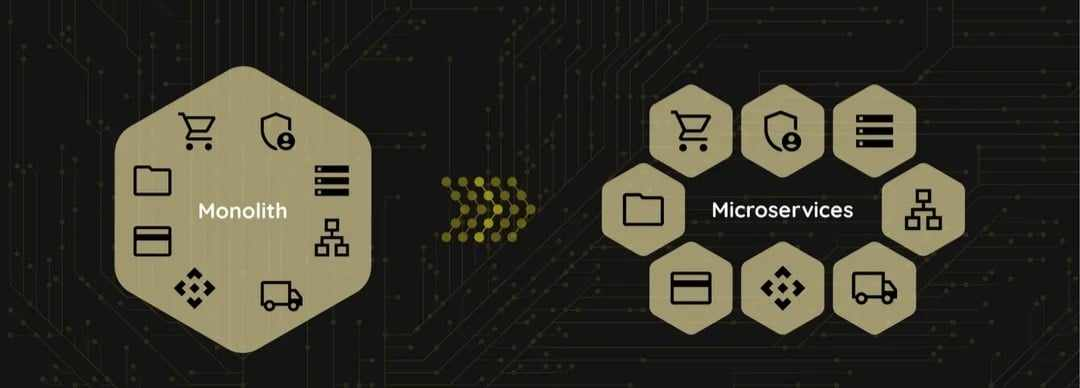
\includegraphics[height = 5cm]{pictures/anh_khac_nhau_giua_kien_truc_nguyen_khoi_va_kien_truc_vi_dich_vu/main.jpg}
 
\caption{Ảnh khác nhau giữa kiến trúc nguyên khối và kiến trúc vi dịch vụ}

\end{figure}



% \subsection{Một số đặc điểm và ưu điểm của kiến trúc vi dịch vụ}

% Kiến trúc vi dịch vụ có nhiều ưu điểm, đặc biệt với các dự án có quy mô lớn và phức tạp.

\begin{itemize}

\item Kiến trúc vi dịch vụ phân chia dự án thành các dịch vụ nhỏ.

\begin{itemize}

\item Giúp việc phát triển và quản lý hệ thống dễ dàng hơn.

\item Tận dụng tài nguyên theo nhu cầu cho từng dịch vụ riêng.

\end{itemize}

\item Các dịch vụ độc lập về nghiệp vụ kinh doanh.

Các nhóm không cần hiểu sâu về mọi khía cạnh kinh doanh. Dẫn tới tốc độ phát triển và tốc độ định giá doanh nghiệp nhanh hơn.

\item Các dịch vụ độc lập về ngôn ngữ lập trình và CSDL

Ví dụ: Mỗi dịch vụ sử dụng ngôn ngữ lập trình và CSDL khác nhau như: NodeJS, Go, Python, Java, CSharp, MongoDB, SQLServer, SQLite, MySQL, PostgreSQL

\begin{figure}[H]

\centering

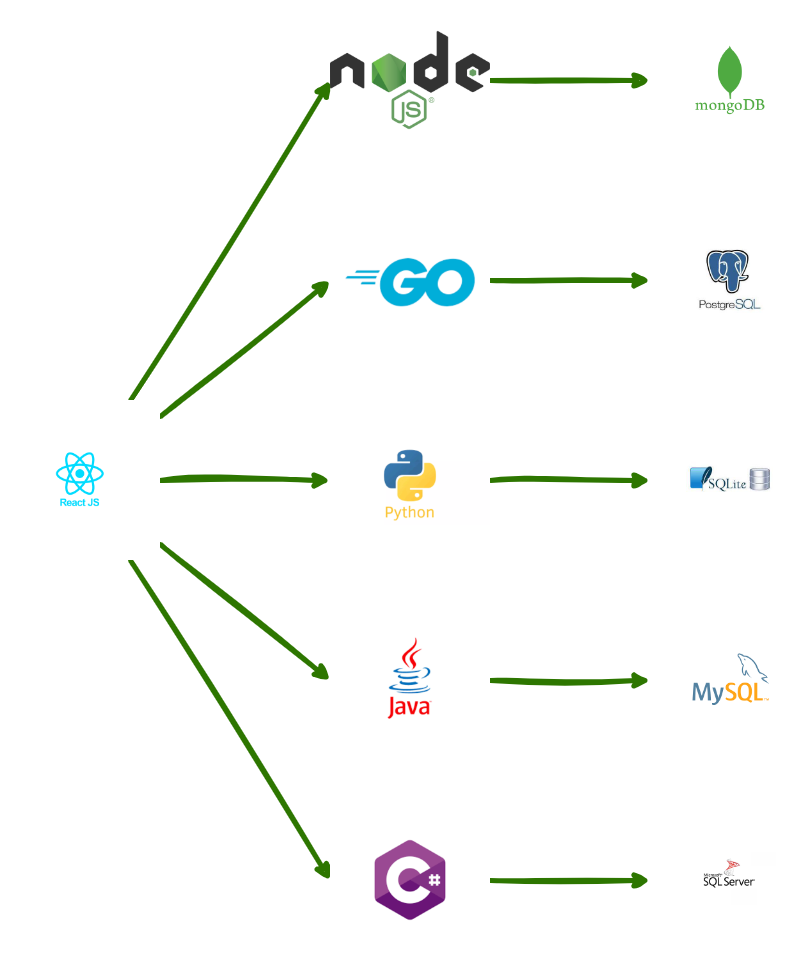
\includegraphics[height = 10cm]{pictures/da_ngon_ngu_va_csdl/main.drawio.png}

\caption{Các dịch vụ độc lập về ngôn ngữ lập trình và CSDL}

\end{figure}

\begin{itemize}

\item Kiến trúc vi dịch vụ sử dụng đa ngôn ngữ và công nghệ khác nhau. Từ đó tận dụng hiệu quả thế mạnh của từng ngôn ngữ, công nghệ phù hợp nhất cho yêu cầu nghiệp vụ cụ thể.

\item Giảm chi phí và thời gian kiểm thử do ít ràng buộc.

\end{itemize}

\item Các dịch vụ độc lập về triển khai hệ thống

Mỗi dịch vụ triển khai độc lập và có thể thay đổi mà không ảnh hưởng đến các dịch vụ khác.

Giảm ràng buộc và tăng tính linh hoạt của hệ thống. Từ đó dễ dàng mở rộng hệ thống.

\item Hệ thống có khả năng chịu lỗi tăng độ tin cậy.

Do các dịch vụ độc lập, nhiều dịch vụ có thể triển khai trong cùng một khả năng kinh doanh để đảm bảo tính sẵn sàng của hệ thống.

\end{itemize}

%%%%%%%%%%%%%%%%%%%%%%%%%%%%%%%%%%%%%

% Các dịch vụ tương tác với nhau qua hạ tầng mạng.



% \subsection{Một số nhược điểm và thách thức của kiến trúc vi dịch vụ}

% Mặc dù kiến trúc vi dịch vụ có nhiều lợi ích, nhưng cũng có nhiều thách thức:

\begin{itemize}

\item Chịu ảnh hưởng của đường truyền mạng.

\item Đồng bộ đồng hồ thời gian.

\item Ràng buộc về thứ tự sự kiện.

\item Tính nhất quán và toàn vẹn của dữ liệu.

\item Khả năng kiểm soát giao dịch.

\item Giám sát giữa các dịch vụ.

\item Bảo mật giao tiếp giữa các dịch vụ.

\item Phát hiện lỗi và sửa lỗi khó khăn, phức tạp hơn.

\item Chi phí xây dựng và quản lý vận hành lớn.

\end{itemize}



%%%%%%%%%%%%%%%%%%%%%%%%%%%%%%%%%%
% \section{Giới thiệu về thiết kế hướng miền}



% Trong quá trình hoạt động kinh doanh, không phải mọi doanh nghiệp đều giữ nguyên mô hình kinh doanh được đưa ra ban đầu của mình. Khi quy mô thị trường thay đổi, việc chuyển đổi mô hình kinh doanh là điều cần thiết. Chuyển đổi kinh doanh như một công cụ linh hoạt giúp các doanh nghiệp có thể phát triển và tồn tại giữa các đối thủ của mình.

Ví dụ:

\begin{itemize}

\item Google bắt đầu như một công cụ tìm kiếm trực tuyến, nhưng sau đó đã mở rộng và thay đổi mô hình kinh doanh qua nhiều dịch vụ và sản phẩm khác nhau như: Dịch vụ đám mây Google Cloud Platform, thư điện tử Gmail, bản đồ Google Maps, lưu trữ tập tin Google Drive, \dots

\item Amazon từ hiệu sách trực tuyến đã trở thành thị trường cho nhà cung cấp khác như: Thương mại điện tử, Dịch vụ đám mây Amazon Web Services (AWS), \dots

\begin{figure}[H]

\centering


\includegraphics[width = 0.5\textwidth]{pictures/kien_truc_vi_dich_vu_cua_amazon/main.png}

\caption{Kiến trúc vi dịch vụ của Amazon}

\end{figure}

\end{itemize}

Đối với những doanh nghiệp không chuyển đổi kinh doanh sẽ không thể tồn tại.

Ví dụ: Gần đây, dịch vụ giao đồ ăn Baemin đã rời khỏi thị trường Việt Nam cũng do sức ép từ các đối thủ khác khiến Baemin khó cạnh tranh trong mảng kinh doanh cốt lõi là giao đồ ăn. Các đối thủ này không chỉ cung cấp dịch vụ giao đồ ăn mà còn có đặt xe, giao hàng,...

\begin{figure}[H]

\centering


\includegraphics[width = 0.5\textwidth]{pictures/baemin/main.png}

\caption{Baemin đã rời khỏi thị trường Việt Nam}

\end{figure}

Hiện nay, các tổ chức doanh nghiệp có nhu cầu chuyển đổi kinh doanh để có thể tồn tại và phát triển khi thị trường thay đổi. Từ đó, đáp ứng nhu cầu của khách hàng, mang lại ưu thế cạnh tranh so với các đối thủ. Do đó, các doanh nghiệp cần hệ thống chuyển đổi nhanh chóng để đáp ứng nhu cầu của mô hình kinh doanh và mong đợi của khách hàng.

$\Rightarrow$ Kiến trúc vi dịch vụ giải quyết những thách thức và hỗ trợ doanh nghiệp chuyển đổi dễ dàng. Tuy nhiên, để xây dựng được kiến trúc vi dịch vụ tốt, cần phải tạo ra các dịch vụ nhỏ phù hợp và duy trì tính độc lập. Trong đồ án này, em sử dụng thiết kế hướng miền để phân tích và xây dựng kiến trúc vi dịch vụ. Thiết kế hướng miền xác định và tổ chức các dịch vụ dựa trên việc hiểu rõ về lĩnh vực kinh doanh, giúp dự án phản ánh đúng các quy trình và quy tắc kinh doanh.

%%%%%%%%%%%%%%%%%%%%%%%%%%%%%%%%%%%%%

%@ \subsection{chưa xong}

% \chapter{Yêu cầu nghiệp vụ}



% \input{contents/yeu_cau_nghiep_vu}

% \subsection {Yêu cầu nghiệp vụ của bài toán phụ}

% \input{contents/yeu_cau_nghiep_vu_cua_bai_toan_phu}

% \subsubsection{Các chức năng tổng quan của bài toán phụ}

% \input{contents/cac_chuc_nang_tong_quan_cua_bai_toan_phu}

% \subsection{Yêu cầu nghiệp vụ chưa xong}

% \input{contents/yeu_cau_nghiep_vu_chua_xong}

%@ \subsection{chưa xong}

%%%%%%%%%%%%%%%%%%%%%%%%%%%%%%%%%%%%%

%@ \subsection{chưa xong}

%! chưa chắc vì mình có mẫu kt

% \chapter{Phân tích thiết kế hệ thống}

% \section{UML Use Case Diagrams}

% \section{UML Activity Diagrams}

% \section{UML Sequence Diagrams}

% \section{UML Class Diagrams}

%@ \subsection{chưa xong}

%%%%%%%%%%%%%%%%%%%%%%%%%%%%%%%%%%%%%

\chapter{Chi tiết và áp dụng thiết kế hướng miền}

\section{Đôi nét về thiết kế hướng miền (DomainDrivenDesign)}

% \input{contents/doi_net_ve_thiet_ke_huong_mien}

% \input{contents/chuyen_gia_nganh}

\section{Định nghĩa miền (Domain)}

% \input{contents/dinh_nghia_mien_domain}


\section{Các mẫu trong thiết kế hướng miền}

% \input{contents/cac_khuon_mau_trong_thiet_ke_huong_mien}

\subsection{Các mẫu chiến lược (Strategic Patterns)}

% \input{contents/gioi_thieu_cac_mau_chien_luoc_strategic}


%%%%%%%%%%%%%%%%%%%%%%%%%%%%%%%%%%
\section{xxxxxxx}
\end{document}
% test 
%%%%%%%%%%%%%%%%%%%%%%%%%%%%%%%%%%

\subsubsection{Miền phụ (Sub - Domain)}

% \input{contents/mien_phu_sub_domain}

\paragraph{Phân loại các miền phụ}

% \input{contents/phan_loai_cac_mien_phu}

\subparagraph{Miền phụ chung (Generic Subdomain)}

% \input{contents/mien_phu_chung_generic_subdomain}

\subparagraph{Miền phụ cốt lõi (Core Subdomain)}

% \input{contents/mien_phu_cot_loi_core_subdomain}

\subparagraph{Miền phụ hỗ trợ (Supporting Subdomain)}

% \input{contents/mien_phu_ho_tro_supporting_subdomain}

% \newpage

\paragraph{Cách xác định các miền phụ}

\input{contents/cach_xac_dinh_cac_mien_phu}

\newpage

\paragraph{Tại sao cần phân loại các miền phụ}

\input{contents/tai_sao_can_phan_loai_cac_mien_phu}

\paragraph{Áp dụng phân loại miền phụ trong đồ án này}

% \input{contents/ap_dung_phan_loai_mien_phu_trong_do_an_nay}

\subsection{Mô hình miền (Domain Models)}

\input{contents/mo_hinh_mien_domain_models}

\subsection{Bối cảnh giới hạn (Bounded Context)}

\input{contents/boi_canh_gioi_han_bounded_context}

\subsection{Ngôn ngữ chung (Ubiquitous Language)}

\input{contents/ngon_ngu_chung_ubiquitous_language}

\subsection{Bản đồ bối cảnh (Context Maps)}

\input{contents/ban_do_boi_canh_context_maps}

\subsection{Chi tiết về các mối quan hệ bối cảnh giới hạn}

\input{contents/chi_tiet_ve_cac_moi_quan_he_boi_canh_gioi_han}

\subsubsection{Mối quan hệ đối xứng (Symmetric Relationship)}

\subparagraph{Mô hình riêng biệt (Separate Ways)}

\input{contents/mo_hinh_rieng_biet_separate_ways}

\subparagraph{Mô hình hợp tác (Partnership)}

\input{contents/mo_hinh_hop_tac_partnership}

\subparagraph{Mô hình hạt nhân chung (Shared Kernel)}

\input{contents/mo_hinh_hat_nhan_chung_shared_kernel}

\end{document}

\paragraph{Mối quan hệ bất đối xứng (Asymmetric Relationship)}

\input{contents/moi_quan_he_bat_doi_xung_asymmetric_relationship}

\subparagraph{Mô hình khách hàng - nhà cung cấp (Customer - Supplier)}

\input{contents/mo_hinh_khach_hang_nha_cung_cap_customer_supplier}

\subparagraph{Mô hình tuân thủ (Conformist)}

\input{contents/mo_hinh_tuan_thu_conformist}

\subparagraph{Mô hình chống đổ vỡ (Anti Corruption Layer)}

\input{contents/mo_hinh_chong_do_vo_anti_corruption_layer}

\paragraph{Mối quan hệ 1 - nhiều (One to Many Relationship)}

\input{contents/moi_quan_he_1_nhieu_one_to_many_relationship}

\subparagraph{Dịch vụ máy chủ mở (Open Host Service)}

\input{contents/dich_vu_may_chu_mo_open_host_srv}

\subparagraph{Ngôn ngữ được xuất bản (Published Language)}

\input{contents/ngon_ngu_duoc_xuat_ban_published_language}

\subsection{Các mẫu kỹ thuật (Tactical Patterns)}

\end{document}

% Giới thiệu về Tactical Patterns

% \input{contents/cac_mau_ky_thuat_tactical}

\subsubsection{Các đối tượng miền (Domain Object)}

% \input{contents/cac_doi_tuong_mien_domain_object}

\paragraph{Đối tượng thực thể (Entities Objects)}

% \input{contents/doi_tuong_thuc_the_entities_objects}

\paragraph{Đối tượng giá trị (Value Objects)}

% \input{contents/doi_tuong_gia_tri_value_objects}

\paragraph{Miền dịch vụ (Service)}

% \input{contents/mien_dich_vu_srv}

% %! Hướng dẫn 7/4

% %! Hướng dẫn 7/5

% \subsubsection{xxxxxxx}

% test

\end{document} % kết thúc

paragraph

% %

% % %! Aggregates/ /

% % Tổng hợp là đối tượng kinh doanh trung tâm trong Bối cảnh giới hạn của chúng ta và xác định phạm vi nhất quán trong bối cảnh giới hạn đó.

% % Tổng hợp = Mã định danh chính của Bối cảnh giới hạn của chúng ta

% \subsubsection{xxxxxxx}

% % test

% \end{document} % kết thúc

% Yêu cầu nghiệp vụ của từng sub

% %

% Sơ đồ if else Đ S

% %

% sub trước model

% %

%%%%%%%%%%%%%%%%%%%%%%%%%%%%%%%%%%%%%

\end{document}

\section{xxxxxxx}

\subsection{xxxxxxx}

\subsubsection{xxxxxxx}

test

% phải có CQRS (Phân chia trách nhiệm truy vấn lệnh)

CQRS là một mẫu kiến trúc riêng biệt có thể được sử dụng kết hợp với thiết kế hướng miền để đạt được những lợi ích nhất định, chẳng hạn như cải thiện hiệu suất và khả năng mở rộng. Tuy nhiên, nó không phải là một yêu cầu để triển khai thiết kế hướng miền.

% phải có event

Ngôn ngữ chung (Ubiquitous Language)

%%%%%%%%%%%%%%%%%%%%%%%%%%%%%%%%%%%%%

\end{document} % kết thúc

Cách tiếp cận này nhấn mạnh tính mô - đun, tính linh hoạt và khả năng phục hồi, cho phép các nhóm làm việc đồng thời trên các phần khác nhau của hệ thống và cho phép phát hành nhanh hơn và thường xuyên hơn. Các vi dịch vụ thường dựa vào các giao thức truyền thông nhẹ, chẳng hạn như REST và thường được triển khai bằng các công nghệ chứa trong bộ chứa như Docker và Kubernetes.

\subsubsection{DevOps Ứng dụng, áp dụng, liên quan,....}

\subsubsection{CI/CD}

\subsubsection{Docker}

\subsubsection{Kubernetes}

%@ Tất cả phải dùng ulli